\documentclass{standalone}
\usepackage{tikz}
\usetikzlibrary{patterns, positioning}
\usepackage[sfdefault]{ClearSans} %% option 'sfdefault' activates Clear Sans as the default text font
\usepackage[T1]{fontenc}

\begin{document}
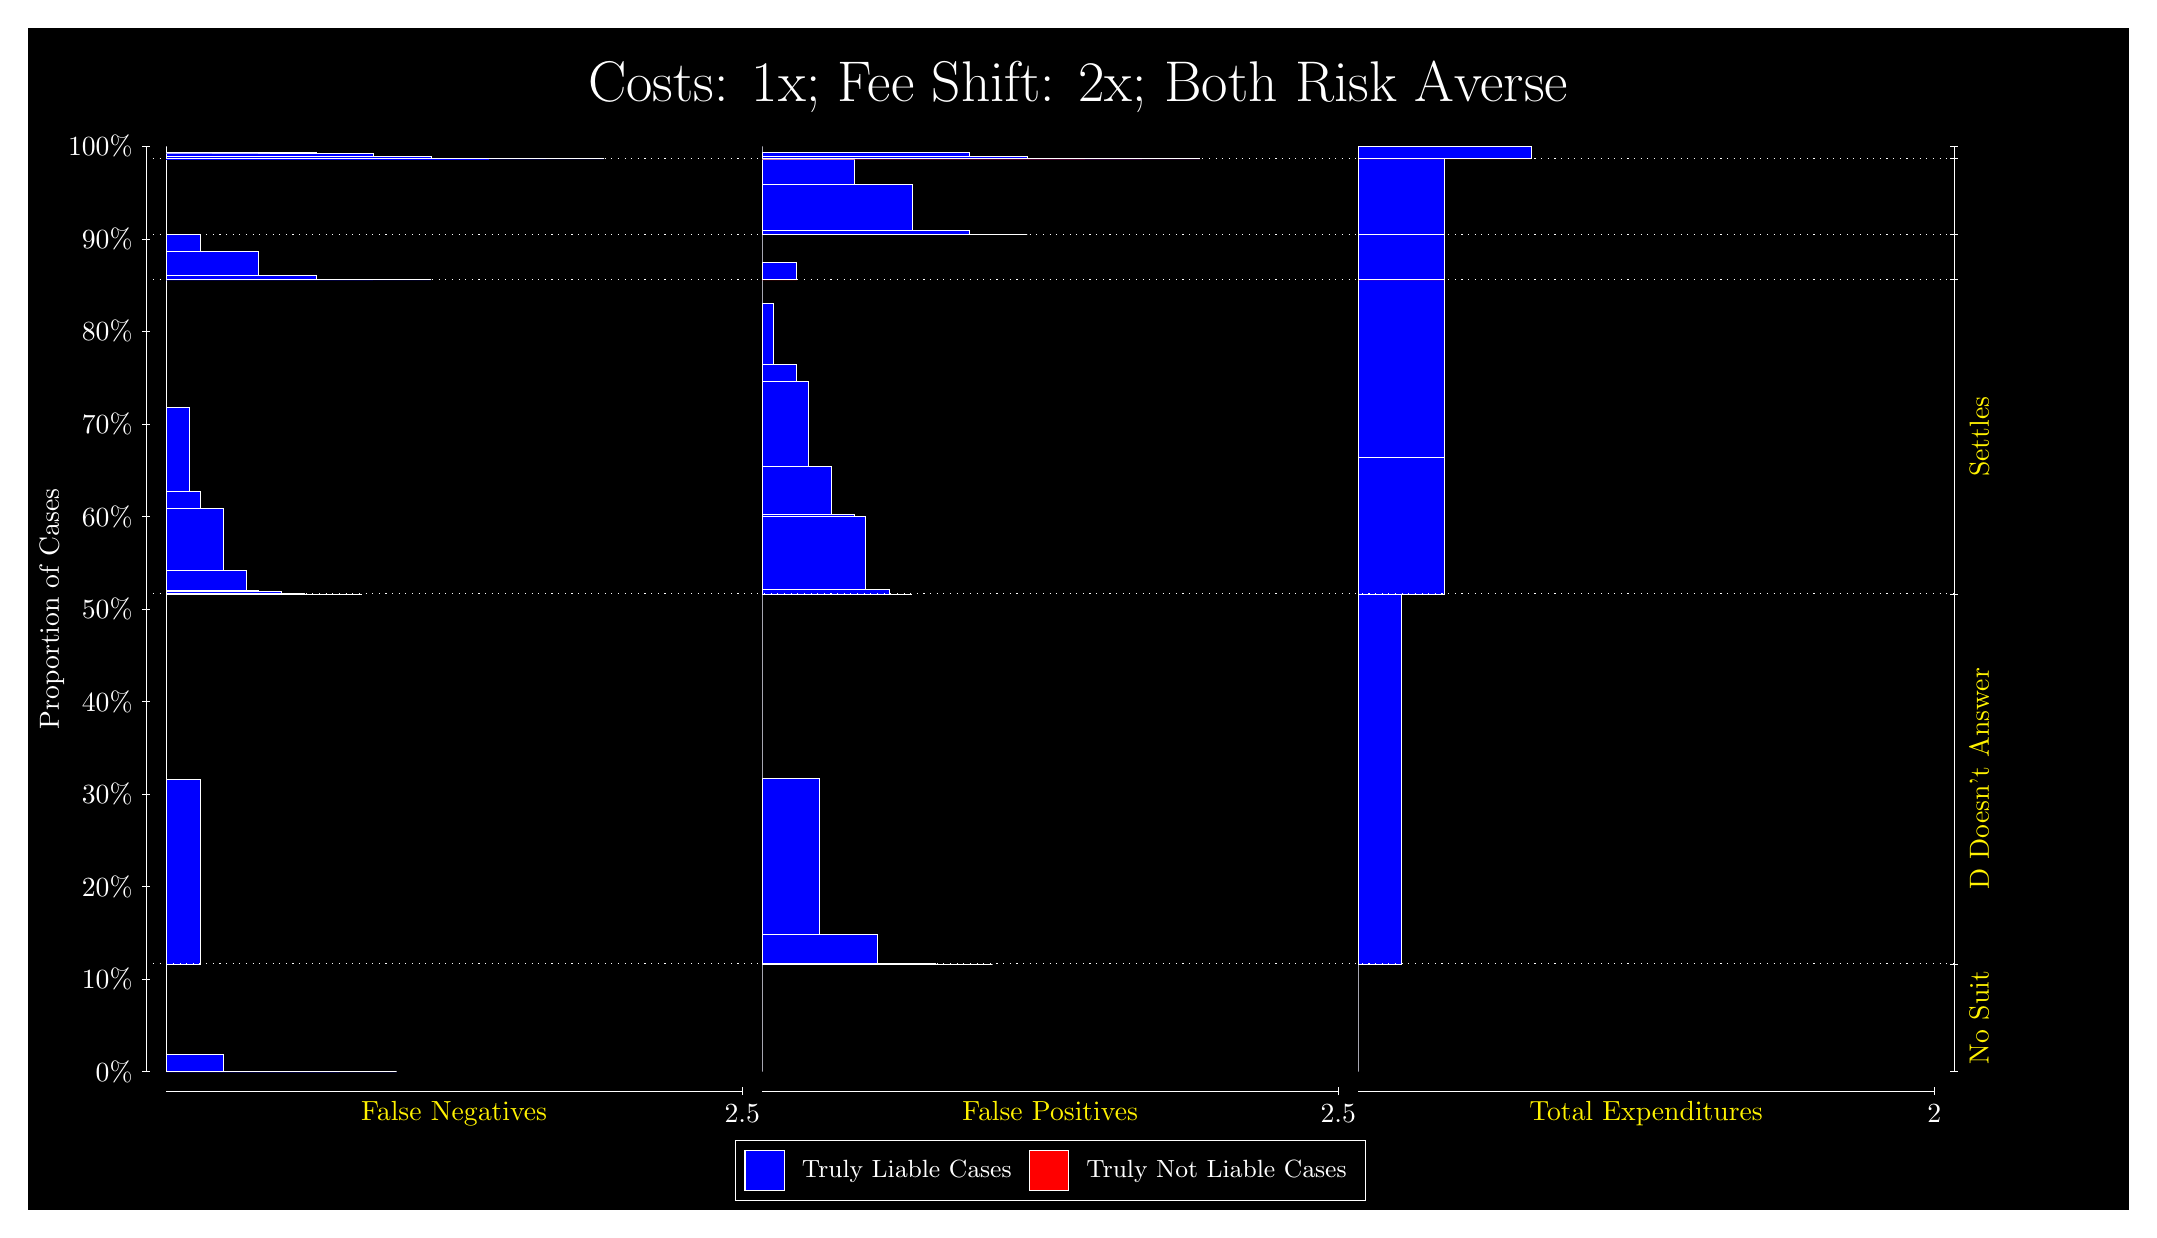
\begin{tikzpicture}
\draw[fill=black] (0,0) rectangle (26.667,15);
\draw[text=white] (0,13.5) rectangle (26.667,15) node[midway] {\huge Costs: 1x; Fee Shift: 2x; Both Risk Averse};
\draw[white, very thin] (1.5,1.75) -- (1.5,13.5);
\node[rotate=90, text=white, anchor=center] at (0.3, 7.625) {Proportion of Cases};
\draw[white, very thin] (1.45,1.75) -- (1.55,1.75);
\node[text=white, anchor=east] at (1.45, 1.75) {0\%};
\draw[white, very thin] (1.45,2.925) -- (1.55,2.925);
\node[text=white, anchor=east] at (1.45, 2.925) {10\%};
\draw[white, very thin] (1.45,4.1) -- (1.55,4.1);
\node[text=white, anchor=east] at (1.45, 4.1) {20\%};
\draw[white, very thin] (1.45,5.275) -- (1.55,5.275);
\node[text=white, anchor=east] at (1.45, 5.275) {30\%};
\draw[white, very thin] (1.45,6.45) -- (1.55,6.45);
\node[text=white, anchor=east] at (1.45, 6.45) {40\%};
\draw[white, very thin] (1.45,7.625) -- (1.55,7.625);
\node[text=white, anchor=east] at (1.45, 7.625) {50\%};
\draw[white, very thin] (1.45,8.8) -- (1.55,8.8);
\node[text=white, anchor=east] at (1.45, 8.8) {60\%};
\draw[white, very thin] (1.45,9.975) -- (1.55,9.975);
\node[text=white, anchor=east] at (1.45, 9.975) {70\%};
\draw[white, very thin] (1.45,11.15) -- (1.55,11.15);
\node[text=white, anchor=east] at (1.45, 11.15) {80\%};
\draw[white, very thin] (1.45,12.325) -- (1.55,12.325);
\node[text=white, anchor=east] at (1.45, 12.325) {90\%};
\draw[white, very thin] (1.45,13.5) -- (1.55,13.5);
\node[text=white, anchor=east] at (1.45, 13.5) {100\%};

\draw[white, very thin] (24.457,1.75) -- (24.457,13.5);
\draw[white, very thin] (24.407,1.75) -- (24.507,1.75);
\node[anchor=west] at (24.407, 1.75) {};
\draw[white, very thin] (24.407,3.1181) -- (24.507,3.1181);
\node[anchor=west] at (24.407, 3.1181) {};
\draw[white, very thin] (24.407,7.8164) -- (24.507,7.8164);
\node[anchor=west] at (24.407, 7.8164) {};
\draw[white, very thin] (24.407,11.807) -- (24.507,11.807);
\node[anchor=west] at (24.407, 11.807) {};
\draw[white, very thin] (24.407,12.385) -- (24.507,12.385);
\node[anchor=west] at (24.407, 12.385) {};
\draw[white, very thin] (24.407,13.343) -- (24.507,13.343);
\node[anchor=west] at (24.407, 13.343) {};
\draw[white, very thin] (24.407,13.5) -- (24.507,13.5);
\node[anchor=west] at (24.407, 13.5) {};

\draw[white, very thin, fill=blue] (1.75,1.75) rectangle (4.6775,1.75);
\draw[white, very thin, fill=blue] (1.75,1.75) rectangle (3.9457,1.75);
\draw[white, very thin, fill=blue] (1.75,1.75) rectangle (3.2138,1.7519);
\draw[white, very thin, fill=blue] (1.75,1.7519) rectangle (2.4819,1.974);
\draw[white, very thin, fill=red] (1.75,1.974) rectangle (1.75,1.974);
\draw[white, very thin, fill=blue] (1.75,1.974) rectangle (1.75,3.1181);
\draw[white, very thin, fill=blue] (1.75,3.1181) rectangle (2.1891,5.4643);
\draw[white, very thin, fill=red] (1.75,5.4643) rectangle (1.75,5.4643);
\draw[white, very thin, fill=blue] (1.75,5.4643) rectangle (1.75,7.8164);
\draw[white, very thin, fill=blue] (1.75,7.8164) rectangle (4.2384,7.8164);
\draw[white, very thin, fill=blue] (1.75,7.8164) rectangle (3.9457,7.8164);
\draw[white, very thin, fill=blue] (1.75,7.8164) rectangle (3.6529,7.8164);
\draw[white, very thin, fill=blue] (1.75,7.8164) rectangle (3.5065,7.8214);
\draw[white, very thin, fill=blue] (1.75,7.8214) rectangle (3.2138,7.8492);
\draw[white, very thin, fill=blue] (1.75,7.8492) rectangle (2.921,7.86);
\draw[white, very thin, fill=blue] (1.75,7.86) rectangle (2.7746,8.116);
\draw[white, very thin, fill=blue] (1.75,8.116) rectangle (2.4819,8.8974);
\draw[white, very thin, fill=blue] (1.75,8.8974) rectangle (2.1891,9.1132);
\draw[white, very thin, fill=blue] (1.75,9.1132) rectangle (2.0428,10.187);
\draw[white, very thin, fill=red] (1.75,10.187) rectangle (1.75,10.187);
\draw[white, very thin, fill=blue] (1.75,10.187) rectangle (1.75,11.807);
\draw[white, very thin, fill=blue] (1.75,11.807) rectangle (5.1167,11.807);
\draw[white, very thin, fill=blue] (1.75,11.807) rectangle (4.3848,11.807);
\draw[white, very thin, fill=blue] (1.75,11.807) rectangle (3.6529,11.864);
\draw[white, very thin, fill=blue] (1.75,11.864) rectangle (2.921,12.163);
\draw[white, very thin, fill=blue] (1.75,12.163) rectangle (2.1891,12.385);
\draw[white, very thin, fill=red] (1.75,12.385) rectangle (1.75,12.385);
\draw[white, very thin, fill=blue] (1.75,12.385) rectangle (2.1891,12.389);
\draw[white, very thin, fill=red] (1.75,12.389) rectangle (1.75,12.389);
\draw[white, very thin, fill=blue] (1.75,12.389) rectangle (1.75,13.343);
\draw[white, very thin, fill=blue] (1.75,13.343) rectangle (7.3123,13.343);
\draw[white, very thin, fill=blue] (1.75,13.343) rectangle (6.5805,13.343);
\draw[white, very thin, fill=blue] (1.75,13.343) rectangle (5.8486,13.345);
\draw[white, very thin, fill=blue] (1.75,13.345) rectangle (5.1167,13.378);
\draw[white, very thin, fill=blue] (1.75,13.378) rectangle (4.3848,13.417);
\draw[white, very thin, fill=blue] (1.75,13.417) rectangle (3.6529,13.421);
\draw[white, very thin, fill=blue] (1.75,13.421) rectangle (3.0674,13.421);
\draw[white, very thin, fill=blue] (1.75,13.421) rectangle (2.921,13.421);
\draw[white, very thin, fill=blue] (1.75,13.421) rectangle (2.3355,13.421);
\draw[white, very thin, fill=red] (1.75,13.421) rectangle (1.75,13.421);
\draw[white, very thin, fill=blue] (1.75,13.421) rectangle (1.75,13.5);
\draw[white, very thin, fill=red] (9.3189,1.75) rectangle (9.3189,1.75);
\draw[white, very thin, fill=blue] (9.3189,1.75) rectangle (9.3189,3.1181);
\draw[white, very thin, fill=red] (9.3189,3.1181) rectangle (12.246,3.1181);
\draw[white, very thin, fill=blue] (9.3189,3.1181) rectangle (12.246,3.1181);
\draw[white, very thin, fill=blue] (9.3189,3.1181) rectangle (11.515,3.121);
\draw[white, very thin, fill=blue] (9.3189,3.121) rectangle (10.783,3.4935);
\draw[white, very thin, fill=blue] (9.3189,3.4935) rectangle (10.051,5.4702);
\draw[white, very thin, fill=blue] (9.3189,5.4702) rectangle (9.3189,7.8164);
\draw[white, very thin, fill=red] (9.3189,7.8164) rectangle (11.222,7.8164);
\draw[white, very thin, fill=blue] (9.3189,7.8164) rectangle (11.222,7.8164);
\draw[white, very thin, fill=red] (9.3189,7.8164) rectangle (10.929,7.8164);
\draw[white, very thin, fill=blue] (9.3189,7.8164) rectangle (10.929,7.8769);
\draw[white, very thin, fill=red] (9.3189,7.8769) rectangle (10.636,7.8769);
\draw[white, very thin, fill=blue] (9.3189,7.8769) rectangle (10.636,8.7992);
\draw[white, very thin, fill=blue] (9.3189,8.7992) rectangle (10.49,8.8241);
\draw[white, very thin, fill=blue] (9.3189,8.8241) rectangle (10.197,9.4358);
\draw[white, very thin, fill=blue] (9.3189,9.4358) rectangle (9.9044,10.51);
\draw[white, very thin, fill=blue] (9.3189,10.51) rectangle (9.758,10.726);
\draw[white, very thin, fill=blue] (9.3189,10.726) rectangle (9.4652,11.507);
\draw[white, very thin, fill=blue] (9.3189,11.507) rectangle (9.3189,11.807);
\draw[white, very thin, fill=red] (9.3189,11.807) rectangle (9.758,11.807);
\draw[white, very thin, fill=blue] (9.3189,11.807) rectangle (9.758,12.028);
\draw[white, very thin, fill=blue] (9.3189,12.028) rectangle (9.3189,12.385);
\draw[white, very thin, fill=red] (9.3189,12.385) rectangle (12.686,12.385);
\draw[white, very thin, fill=blue] (9.3189,12.385) rectangle (12.686,12.385);
\draw[white, very thin, fill=blue] (9.3189,12.385) rectangle (11.954,12.432);
\draw[white, very thin, fill=blue] (9.3189,12.432) rectangle (11.222,13.012);
\draw[white, very thin, fill=blue] (9.3189,13.012) rectangle (10.49,13.339);
\draw[white, very thin, fill=blue] (9.3189,13.339) rectangle (9.758,13.343);
\draw[white, very thin, fill=red] (9.3189,13.343) rectangle (14.881,13.343);
\draw[white, very thin, fill=blue] (9.3189,13.343) rectangle (14.881,13.343);
\draw[white, very thin, fill=red] (9.3189,13.343) rectangle (14.149,13.343);
\draw[white, very thin, fill=blue] (9.3189,13.343) rectangle (14.149,13.343);
\draw[white, very thin, fill=red] (9.3189,13.343) rectangle (13.417,13.343);
\draw[white, very thin, fill=blue] (9.3189,13.343) rectangle (13.417,13.346);
\draw[white, very thin, fill=red] (9.3189,13.346) rectangle (12.686,13.346);
\draw[white, very thin, fill=blue] (9.3189,13.346) rectangle (12.686,13.379);
\draw[white, very thin, fill=blue] (9.3189,13.379) rectangle (11.954,13.419);
\draw[white, very thin, fill=blue] (9.3189,13.419) rectangle (11.222,13.422);
\draw[white, very thin, fill=blue] (9.3189,13.422) rectangle (10.49,13.422);
\draw[white, very thin, fill=red] (9.3189,13.422) rectangle (9.9044,13.422);
\draw[white, very thin, fill=blue] (9.3189,13.422) rectangle (9.9044,13.422);
\draw[white, very thin, fill=blue] (9.3189,13.422) rectangle (9.758,13.422);
\draw[white, very thin, fill=red] (9.3189,13.422) rectangle (9.3189,13.422);
\draw[white, very thin, fill=blue] (9.3189,13.422) rectangle (9.3189,13.5);
\draw[white, very thin, fill=red] (16.888,1.75) rectangle (16.888,1.75);
\draw[white, very thin, fill=blue] (16.888,1.75) rectangle (16.888,3.1181);
\draw[white, very thin, fill=red] (16.888,3.1181) rectangle (17.437,3.1181);
\draw[white, very thin, fill=blue] (16.888,3.1181) rectangle (17.437,7.8164);
\draw[white, very thin, fill=red] (16.888,7.8164) rectangle (17.986,7.8164);
\draw[white, very thin, fill=blue] (16.888,7.8164) rectangle (17.986,9.5493);
\draw[white, very thin, fill=red] (16.888,9.5493) rectangle (17.986,9.5493);
\draw[white, very thin, fill=blue] (16.888,9.5493) rectangle (17.986,11.807);
\draw[white, very thin, fill=red] (16.888,11.807) rectangle (17.986,11.807);
\draw[white, very thin, fill=blue] (16.888,11.807) rectangle (17.986,12.385);
\draw[white, very thin, fill=red] (16.888,12.385) rectangle (17.986,12.385);
\draw[white, very thin, fill=blue] (16.888,12.385) rectangle (17.986,13.343);
\draw[white, very thin, fill=red] (16.888,13.343) rectangle (19.083,13.343);
\draw[white, very thin, fill=blue] (16.888,13.343) rectangle (19.083,13.5);
\draw[white, dotted] (1.5,3.1181) -- (24.457,3.1181);
\draw[white, dotted] (1.5,7.8164) -- (24.457,7.8164);
\draw[white, dotted] (1.5,11.807) -- (24.457,11.807);
\draw[white, dotted] (1.5,12.385) -- (24.457,12.385);
\draw[white, dotted] (1.5,13.343) -- (24.457,13.343);
\draw[white, very thin] (1.75,1.5) -- (9.0689,1.5);
\node[text=yellow, anchor=north] at (5.4094, 1.5) {False Negatives};
\draw[white, very thin] (9.0689,1.45) -- (9.0689,1.55);
\node[text=white, anchor=north] at (9.0689, 1.45) {2.5};

\draw[white, very thin] (9.3189,1.5) -- (16.638,1.5);
\node[text=yellow, anchor=north] at (12.978, 1.5) {False Positives};
\draw[white, very thin] (16.638,1.45) -- (16.638,1.55);
\node[text=white, anchor=north] at (16.638, 1.45) {2.5};

\draw[white, very thin] (16.888,1.5) -- (24.207,1.5);
\node[text=yellow, anchor=north] at (20.547, 1.5) {Total Expenditures};
\draw[white, very thin] (24.207,1.45) -- (24.207,1.55);
\node[text=white, anchor=north] at (24.207, 1.45) {2};

\node[text=yellow, centered, rotate=90] at (24.777, 2.4341) {No Suit};
\node[text=yellow, centered, rotate=90] at (24.777, 5.4673) {D Doesn't Answer};
\node[text=yellow, centered, rotate=90] at (24.777, 9.8115) {Settles};




\draw (12.978300999999998,1.5) node[draw=none] (baseCoordinate) {};
\begin{scope}[align=center]
        \matrix[scale=0.5, draw=white, below=0.5cm of baseCoordinate, nodes={draw}, column sep=0.1cm]{
            \node[rectangle, draw, minimum width=0.5cm, minimum height=0.5cm, fill=blue] {}; &
            \node[draw=none, font=\small, text=white] (B) {Truly Liable Cases}; &
            \node[rectangle, draw, minimum width=0.5cm, minimum height=0.5cm, fill=red] {}; &
            \node[draw=none, font=\small, text=white] (B) {Truly Not Liable Cases}; \\
            };
\end{scope}

\end{tikzpicture}
\end{document}